\chapter{Architectural description}
	This chapter will revolve around the final architecture of the prototype created during this project. In our definition of architecture, we have choosen to follow the definition carved out by
	Len Bass, Paul Clements and Rick Kazman. 
	\newline
	\newline
	"The software architecture of a program or computing system is the stucture of structures of the system, which comprise software elements, the externally visible properties of those elements, and the relationships between them''\cite[p. 3]{bib:archi}
	\newline
	\newline
	In the first part of this chapter we will focus on architectural drivers and viewpoints, before we move on to discussing how the Android platform behaves on the frontend part of our application, how we tried to utilize these Android features and how the activity flow of our application is set up. We will end this chapter with the architectural tactics and patterns implemented in our application. 
	
\section{Architectural Drivers}
	From the nature of the assignment and the requirements received from the customer, we decided that \highlight{Security} had to be one of our quality attributes. After the first couple of meetings with the customer, it became clear that usability also was something of interest to them, and we decided to add \highlight{Usability} to our quality attributes as well. It should however be noted that all of the quality attributes specified in Len Bass's book 'Software Architecture in Practice'\cite{bib:archi} had their place within this project. Especially \highlight{Modifiability}, though not one of our main attributes, was given a fairly large amount of consideration in order to ease development at later stages of the project. The reason as to why Modifiability was not one of our main attributes comes down to the expected lifespan of the prototype, which in this case is largely dependent on the success of the project, and what prospects the customer sees when presented with the final prototype and documentation. However, the project revolves around making a prototype and documenting the steps taken to complete that process, and it is therefore safe to assume that the lifespan of the prototype will be relatively short. 

\section{Architectural viewpoints}
The "4+1 view model'' \cite{bib:vm} by Philippe Kruchten suggest four different views, logical, process, development and physical. In the case of XOXOmail we are going to use the logical, process and development view. The rationale behind removing the physical view is that XOXOmail will run on a single physical device and only utilize one process. A security view, describing the layers of security, will be added instead.

\subsection{Development view (Subsystem decomposition)}
The development view focuses on software modules and subsystems. These subsystems/modules are organized in a hierarchy of layers where each layer provides a well-defined interface to layers above. 
\newline
\newline
``The complete development architecture can only be described when all the elements of the software have been identified. It is, however, possible to list the rules that govern the development architecture: partitioning, grouping, visibility'' \cite{bib:vm}. 
\newline
\newline
Figure \ref{fig:developmentview} at page \pageref{fig:developmentview} shows the Backend Service Connects to all parts of our app. The main focus of this view is to show that it is also the connector to the external parts of the app, which in our case is just a mail gateway. The final goal will be to connect to Thales' gateway, but as long as the gateway comply with the standards of \gls{smtp} and \gls{pami} there should be no problem.

\begin{figure}[H]
	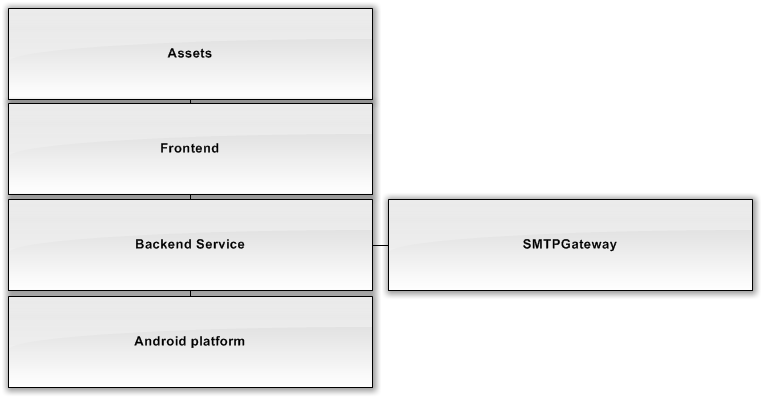
\includegraphics[width=\textwidth]{developmentview.png}
	\caption{Development view}
	\label{fig:developmentview}
\end{figure}

\subsection{Logical view (Object oriented decomposition)}\label{ch:logicalview}
``The logical architecture primarily supports the functional requirements --- what the system should provide in terms of services to its users. The system is decomposed into a set of key abstractions, taken from the problem domain, in the form of objects or object classes''\cite{bib:vm}. 
\newline
\newline
A common way to represent this view is with a class diagram that shows a set of classes and their relationships. We have however used a slightly modified variant, in order to make all the figures more readable.
\subsubsection{Backend}
\begin{figure}[H]
	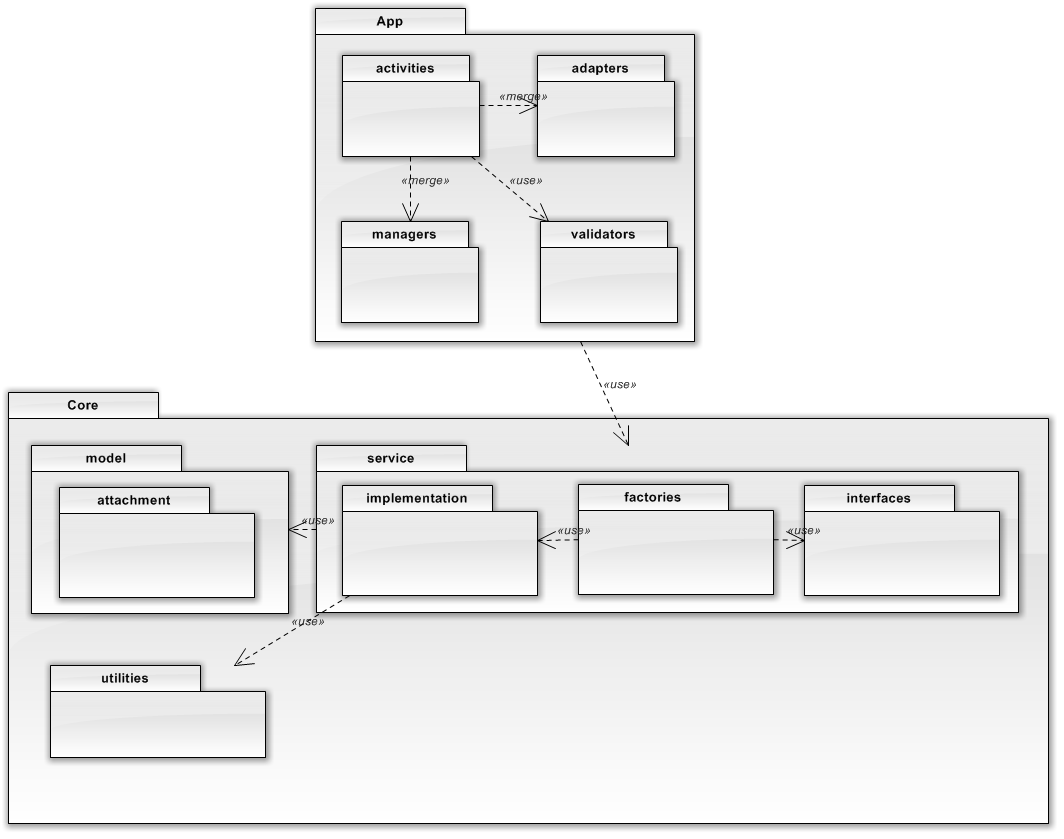
\includegraphics[width=\textwidth]{packageDiagram.png}
	\caption{The logical package view of the architecture}
	\label{fig:logicalpackview}
\end{figure}
\newpage
Figure \ref{fig:logicalpackview} shown at page \pageref{fig:logicalpackview}, shows a package overview over the project backend. Though rather rudimentary, it shows the basic structure of the architecture and the most common communication paths between packages. On thing to note, is that in order to add a new service to the architecture, one would need to implement three different objects, a factory for creating the service, an interface describing the service, and the service implementation itself.
\newline
\newline
In the case of XOXOmail, we planned out four different services, the \highlight{NetworkService}~(Fig.~\ref{fig:logicalnetworkpackview}~p.~\pageref{fig:logicalnetworkpackview}), \highlight{PersistenceService}~(Fig.~\ref{fig:logicalpersistencepackview}~p.~\pageref{fig:logicalpersistencepackview}), \highlight{HALService} and \highlight{SecurityService}. The two latter was though never used, and their diagrams are therefore omitted here, alongside the diagram for our \textsc{Utilities} package. The structure of our models can be seen in figure~\ref{fig:logicalmodelpackview} at page \pageref{fig:logicalmodelpackview}

\begin{figure}[H]
	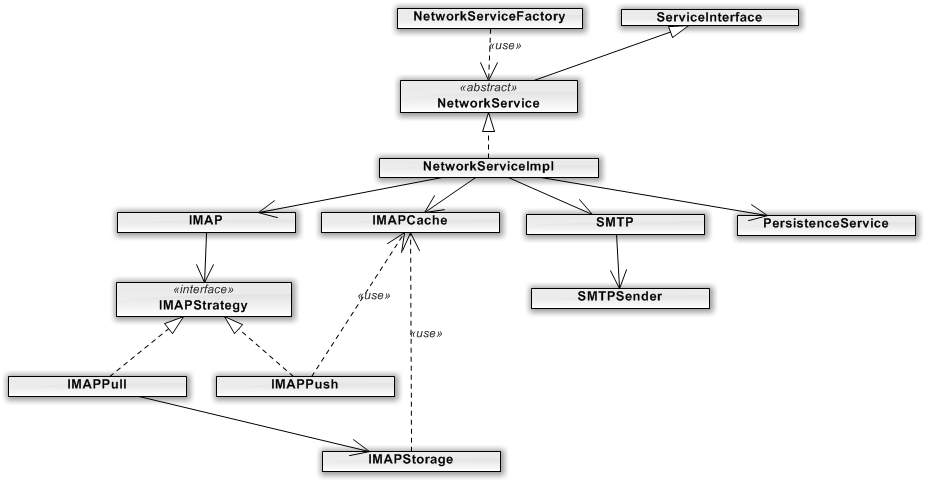
\includegraphics[width=\textwidth]{NetworkService.png}
	\caption{The logical view of the NetworkServicePackage}
	\label{fig:logicalnetworkpackview}
\end{figure}
\begin{figure}[H]
	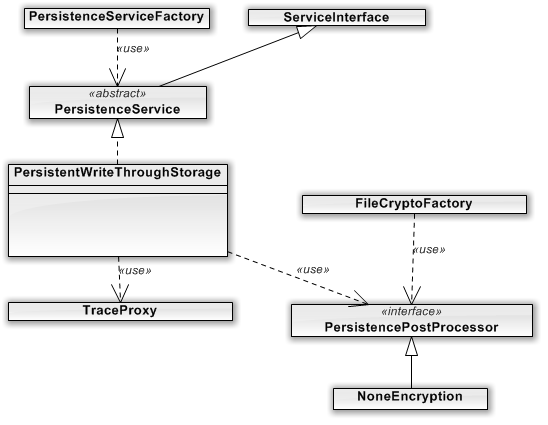
\includegraphics[width=\textwidth]{persistenceService.png}
	\caption{The logical view of the PersistenceService}
	\label{fig:logicalpersistencepackview}
\end{figure}
\begin{figure}[H]
	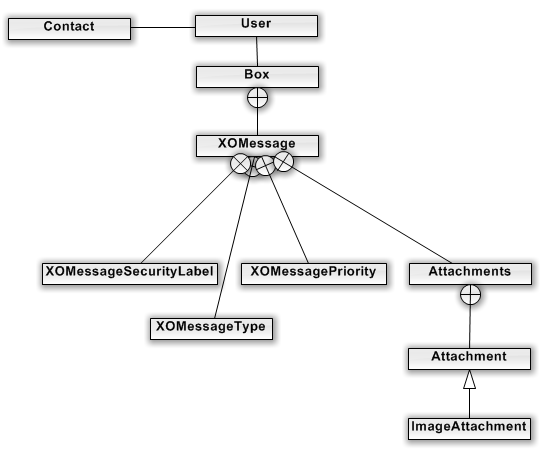
\includegraphics[width=\textwidth]{modelPackage.png}
	\caption{The logical view of the model package}
	\label{fig:logicalmodelpackview}
\end{figure}

The intended purpose of each of the different services is somewhat given by their respective names, but in order to avoid any ambiguity there will be a short recap of their purpose.
\begin{description}
	\item[NetworkService] The \highlight{NetworkService}'s reponsebility is to provide the core functionality of sending and receiving messages. 
	\item[PersistenceService] The \highlight{PersistenceService}'s responsebility is to keep track of objects being changed, and reflect these changes in a persistent way in case of system failure, or if the application is shut down. 
\end{description}

\subsubsection{Frontend}
	\begin{figure}[H]
		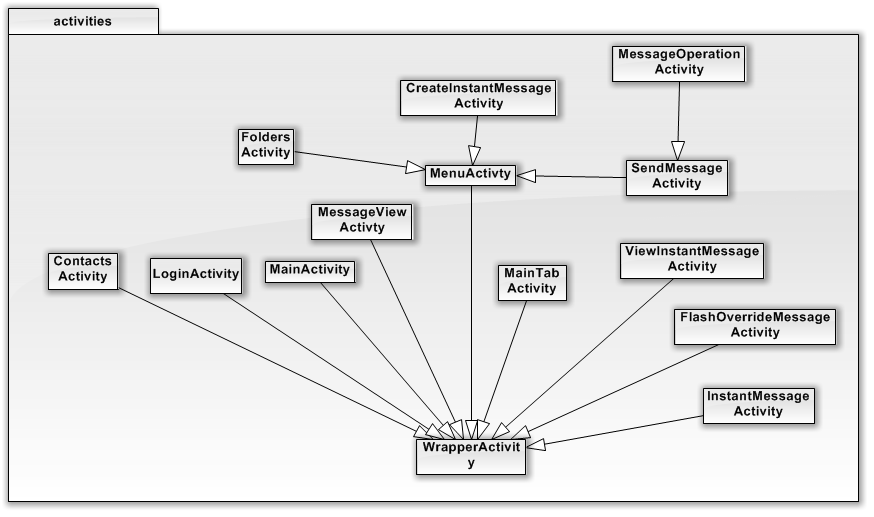
\includegraphics[width=\textwidth]{FrontendClasses.png}
		\caption{The logical view of the frontend activities package}
		\label{fig:logicalfrontpackview}
	\end{figure}	
	
\subsection{Process view}
The process view is concerned with how different tasks bind together to form one executable unit. More specifically, the communication between threads/processes and on which thread/process a task is executed. We will differentiate between major and minor tasks, where major tasks are architectural elements open through a public interface, and minor tasks being tasks introduced in order to implement some functionality in one class or module.
In figure \ref{fig:processview} at page \pageref{fig:processview}, you can differentiate between minor and major tasks by looking at the \highlight{smtp} branch of \highlight{NetworkService}, here \highlight{SMTPSender} is a minor task, while both \highlight{SMTP} and \highlight{NetworkService} is considered major tasks. 

\begin{figure}[H]
	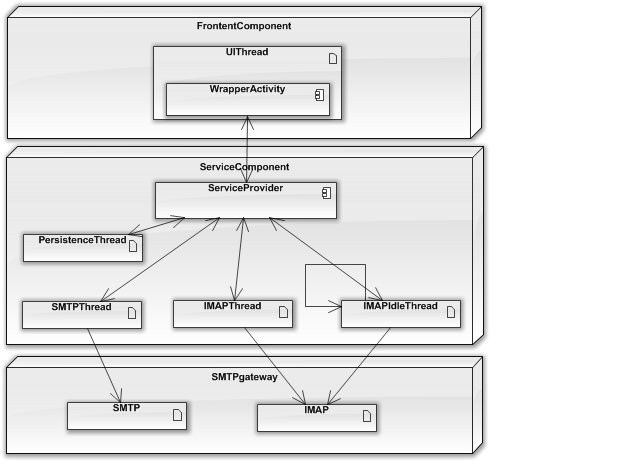
\includegraphics[width=\textwidth]{processview.png}
	\caption{Process view}
	\label{fig:processview}
\end{figure}

One thing to note about the communications paths is that almost all communication between the \highlight{frontent component} and \highlight{service component} is between two wrapper classes, \highlight{WrapperActivity} at the frontend, and \highlight{ServiceProvider} at the backend. The services under the \highlight{ServiceProvider} does however implement the \highlight{observable} pattern, which opens up some alternative communications paths for callbacks.

\subsection{Security view}
The security view is concerned with how the system as a whole is secured. This involves intercommunication, storage and communication with external sources. The view is not however concerned about implementation, just the layers of security.
See figure \ref{fig:securityview} at page \pageref{fig:securityview}.

\begin{figure}[H]
	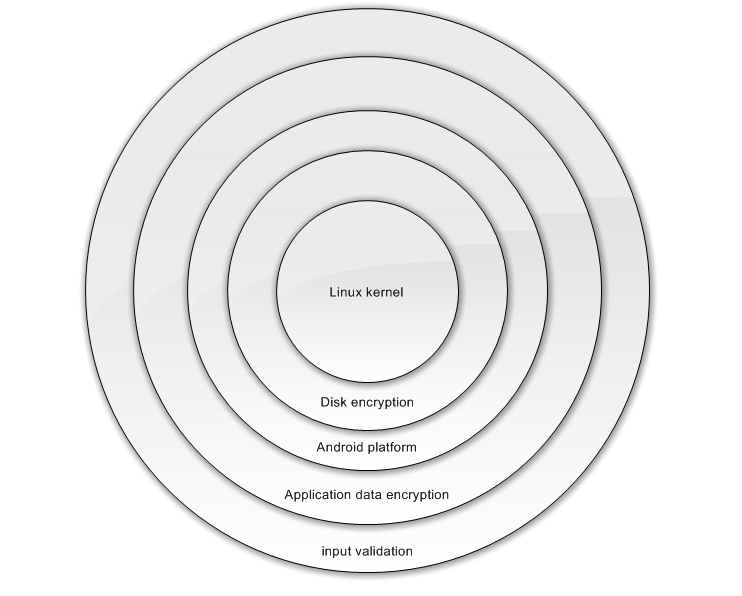
\includegraphics[width=\textwidth]{securityview.png}
	\caption{Security view}
	\label{fig:securityview}
\end{figure} \hfill
\newline
\newline
\textbf{The Linux kernel} provides us with a user-based permissions model and process isolation, which ensures that another process cannot access the memory of XOXOMail during runtime.
\newline
\newline
\textbf{Disk encryption}, is feature provided by the Android platform, which encrypts the whole Android device using \gls{aes} with \gls{cbc} and \gls{essiv2}.\cite{bib:crypto}
\newline
\newline
\textbf{Android platform}, most of the security features provided by the Android platform utilize the Linux kernel. The application sandbox feature is one of these, and since it is located at the kernel level, it is hard to circumvent.
\newline
\newline
\textbf{Application data encryption} is a response to the possibility of rooted devices. Normally an Android application will not run with root access on the device, this however is not the case on rooted devices. In which case the application and user will have full access to all applications and all application data. By adding our own encryption layer with the key stored off-device we can ensure data security even with root access to the phone\cite{bib:tech}. The encryption we opted for is an \gls{aes} based encryption with a user-password derived key by \gls{pbsha}.
Regarding communication with external resources as a mail server, it will be done over a secure communication channel providing \gls{ssl1} or \gls{tls}. 
\newline
\newline
\textbf{Input validation} is always necessary in order to provide a secure service. All input to the XOXOMail application should be validated, this includes received mail, user-input etc. For message validation we planned on using \gls{emims} signing and verification provided by an Android ported version of \gls{bouncy} called \gls{spongy}, this was never implemented due to time restrictions. 

\section{Frontend}

\subsection{Introduction}
The section will describe the process of creating the user interface, the Android guidelines for creating an application, out take on these guidelines, and how the user interface turned out including the rationale behind the decision made.
%This section will describe the process of creating the user interface, how the Android framework has specified implementing an app and what elements we conformed to in this specification, and how the %user interface looks like and why.

\subsection{The design process}
This section will outline the design process from requirements and prototyping to implementation and testing.

\subsubsection{Planning from the requirements}
At the start, we looked at the requirements to get an overview of what views we needed and the basic functionality each view should have. 

\subsubsection{Prototyping}
Then, we started to create simple sketches of each view, what components each view should consist of and the layout of each view. We also tried to outline the flow between the views. In this phase we had several suggestions as to the layout and main form of navigation. After some consideration we decided on the tab navigation pattern.
%We settled for one method, namely the tab navigation pattern.
\newline
\newline
After the inital sketches we created an interactive prototype using the online prototyping tool FLUIDUI SOURCE. This enabled us to share our thoughts with the customer and give them an early insight into what direction we were headed with the design.
%We also tried using an online prototyping tool FLUIDUI SOURCE that we shared with the customer to give them an early insight into what direction we were headed with the design. 

\subsubsection{Continuous feedback and implementation}
We continued to keep an open dialog with the customer about what they wanted regarding functionality and feedback from the user interface. The implementation was split up in iterations according to the sprints where we implemented functionaliy that we had planned and the customer gave feedback at the end of each sprint and demonstration. 
\newline
\newline
Even though we had tried to dig into the Android framework prior to the implementation, as outlined in section \ref{subsec:androidframework}, we did not have a full overview over what was possible in the framework. Implementing each view as we wanted became a process of trial and error and we learnt a lot during this process. We tried to stick to Android's specified way of doing things and using the built-in architecture and components, to avoid the effort of creating custom components from scratch, as we did not have that much time available. 

\subsubsection{Testing}
We tested the app continously throughout the sprints, as well as conducting a final black-box functional testing as described in section \ref{subsec:functionaltesting}. We also conducted a usability study to investigate whether we had succeeded in creating a usable user interface. These tests, in addition to the results, are described in section \ref{subsec:usabilitytesting}.

\subsection{The Android framework}\label{subsec:androidframework}
This section will cover the Android frameworks's guidelines regarding the organization of an application, and our take on these guidelines. 
%This section describes the way the Android framework has specified of organizing the application, which we have tried to follow.

\subsubsection{External resources}
The user interface elements, ranging from whole views to the structure and look of a single list element, are defined in \gls{xml} and stored external to the application. An Android project contains a folder named “res” where all external resources are placed. User interface elements are stored in a sub folder called “layouts”. Other resources, e.g. colors or images, are stored inside separate sub folders. The advantage of declaring the user interface and other resources in \gls{xml} is that it enables decoupling of the presentation of the application and the code that controls the application.
\newline
\newline
All resources must be assigned an \gls{id} if they are to be referenced to in the application code. All resource \gls{id}s are defined as public constants in the project's R.class, which is a class that is automatically generated during build and contains subclasses for the types of resources where we have defined at least one resource, e.g. R.layout (for user interface elements) or R.color (for definition of colors). The resources can be referenced both inside other resources and in the application code.
\newline
\newline
We also wanted to use styles, which are collections of properties specifying the look of a layout or a component. It can be compared to the mindset of \gls{css}. The reason behind using styles and fixed color definitions would be to ensure consistent appearance across the application. 

\subsubsection{Activities}
Activities are components that provide a view that the user can interact with, and are classes written in Java. Each activity has a window where the user interface is drawn. One activity is specified as the main activity and is the start screen of the application. Each activity can start another activity to perform different actions. The activities inflate the \gls{xml} layouts to form the user interface and controls the behaviour of the elements. It is also possible to create layout elements programmatically, but we have chosen not to do this as we want the decoupling mentioned above.
\newline
\newline
An activity is always in one of four possible states \cite{bib:aas}:
\begin{itemize}
\item{}Active/running: When the activity is in the foreground of the screen
\item{}Paused: When the activity has lost focus but is still visible
\item{}Stopped: When the activity is completely obscured by another activity
\item{}If an activity is paused or stopped, it is likely that the system asks the activity to finish or just kill its process, hence drops it from memory. It then has to be restarted completely.
\end{itemize}

The life cycle of an activity can be seen in figure \ref{fig:lifecycle} at page \pageref{fig:lifecycle}.
\begin{figure}
	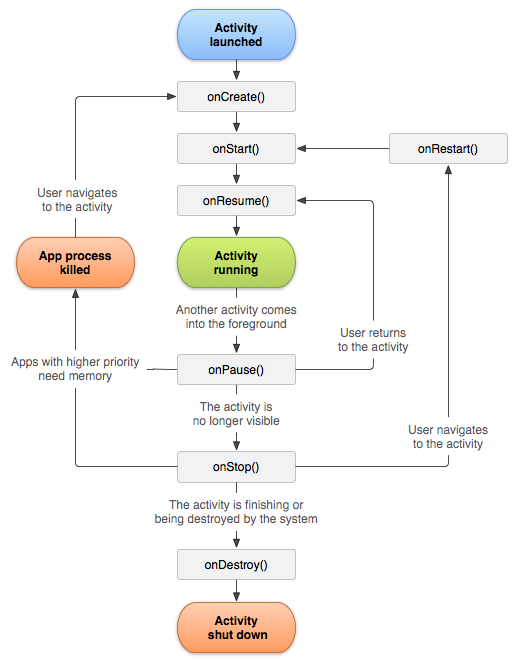
\includegraphics[width=\textwidth]{activity_lifecycle}
	\caption{Activity life cycle \cite{bib:alc}}
	\label{fig:lifecycle}
\end{figure}

All the methods starting with 'on' (onCreate etc.) can be overwritten to administrate what the application should do in the changes of state.

\subsubsection{The Android manifest}
The Android manifest \cite{bib:aman} is what binds the application together. It is defined in \gls{xml} and details the structure and metadata of the application, its components and requirements. The manifest needs to have nodes for each of the components, which in our case are activities, services and broadcast receivers. Relevant metadata is the application name, icon and theme. The manifest also declares the permissions the application needs to access protected parts of the \gls{api} and interact with other applications.

\subsubsection{Supporting different hardware and internationalization}
By conforming to using external resources on can easily build applications that support differences such as varying screen sizes and languages. For example, it is possible to create a low, medium and high \gls{dpi} version of an image and Android will select the correct version based on the screen size. Android can pick layouts based on the screen orientation, where the possibilities are that the phone is an portrait or landscape mode. It is also possible to have Android decide what language to use based on location, but this is not relevant to this project. 

\newpage
\subsection{Our solution}

This chapter describes our solution with regards to the user interface and the reason behind the most important choices. The evolution of the user interface during the different sprints is documented in the sprint chapters.

\subsubsection{The most important design choices}

\paragraph{The tab navigation system}\hfill
\newline
The choice of a main form of navigation fell on a tabbed system, as seen in figure \ref{fig:frontend_inbox} on page \pageref{fig:frontend_inbox}. The initial thought behind using this form of navigation was that we got an easy way of navigating around the different views and a quick view of the available views.
At a later point we figured out that the tab navigation is supposed to be used for switching between different views of the same type, which is not the case in our app. We also ran into some problems with the built-in Android tab component. Unfortunately this was at a point too late to conduct any drastical changes, and we think that the solution is well enough suited for this prototype.

\begin{figure}[h!]
\begin{center}
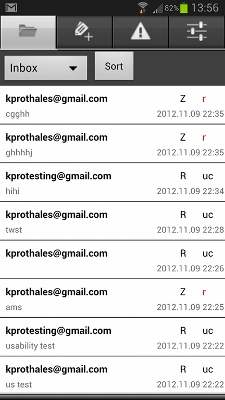
\includegraphics{inbox_final}
\end{center}
\caption{Inbox view} \label{fig:frontend_inbox}
\end{figure}

\paragraph{The inbox}\hfill
\newline
The inbox and message folders are composed in an identical way. We used a list where we specified a custom layout of each message item in the list, as seen in figure \ref{fig:frontend_inbox} on page \pageref{fig:frontend_inbox}. All the information on each item was requested from the customer, and we tried to make it look like a the standard way of listing mails 
in an inbox. We used abbreviations for the security labels (e.g. the Z and R) and priorities (e.g. r and uc) as specified by the customer because of the limited space of each message item. We also added the common clip icon to inform the user that the message has files attached. 

\paragraph{Messages}\hfill
\newline
If the user clicks an item in the message list he/she is sent to the view for showing the full information of the message, as seen in figure \ref{fig:frontend_message} on page \pageref{fig:frontend_message}. We chose to list the military messaging attributes in a separate box to easy give an overview of them. We originally had a more elaborate plan as to show the attachments, but ended up with a button the opens a dialog box as this was easier to implement, and we were short on time. 
%We originally planned to have a fancy function that showed the attachments, but ended up with a button that opens a dialog box as this was easier to implement and was created towards the end of the %project. 
The common choices of replying to and forwarding a message, as well as buttons with arrows to browse between the messages are placed at the bottom of the screen.

\begin{figure}[h!]
\begin{center}
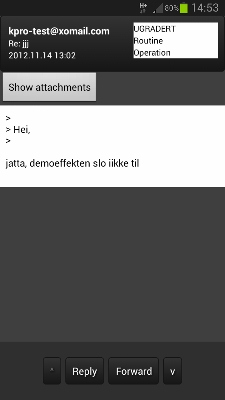
\includegraphics{message_final}
\end{center}
\caption{Message view} \label{fig:frontend_message}
\end{figure}


\paragraph{Sending a message}\hfill 
\newline
The view for sending messages is broken down into the logical part of a message conforming to the \gls{mmhs} standards, as shown in figure \ref{fig:frontend_messagesend} on page \pageref{fig:frontend_messagesend}.
%The view for sending a message is composed of what we think is the logical way of entering the information, as shown in figure \ref{fig:frontend_messagesend} on page \pageref{fig:frontend_messagesend}.
The selection of military attributes are realized by the use of the Android component spinner, which from a behavioural aspect looks like a drop-down menu.
%We used the same way of selecting the military attributes, namely to use what Android calls a spinner, a kind of a drop-down list with all the available attributes. 
As the diligent reader may have noticed, there is not button for sending the message. This is however just because view is bigger then the screen, and scrolling down to the bottom of the view would reveal the button. 
%Though the button for sending is not visible in the screenshot, because the screen is scrollable.

\begin{figure}[h!]
\begin{center}
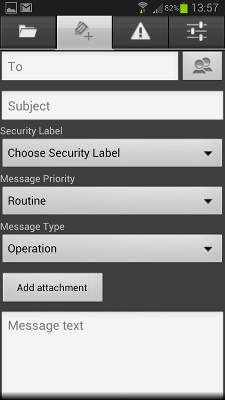
\includegraphics{sendmessage_final}
\end{center}
\caption{Sending message view} \label{fig:frontend_messagesend}
\end{figure}

\paragraph{Instant message}\hfill
\newline
The requirement for instant messages was that it should be possible to send an instant message by using three or less user actions. We thought about different ways of doing this, but ended up with the solution that is shown in figure \ref{fig:frontend_instamessage} on page \pageref{fig:frontend_instamessage}.
One has to set the standard attributes for the instant message in the settings, thus requiring a couple of actions before being able to send an instant message, but after this one can send instant messages with no more than three clicks (e.g. push the instant message tab, enter text and push send). 

\begin{figure}[h!]
\begin{center}
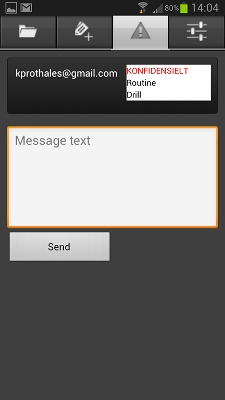
\includegraphics{instantmessage_final}
\end{center}
\caption{Sending instant message view} \label{fig:frontend_instamessage}
\end{figure}

\subsubsection{Activities and flow between them}

\begin{figure}[h!]
	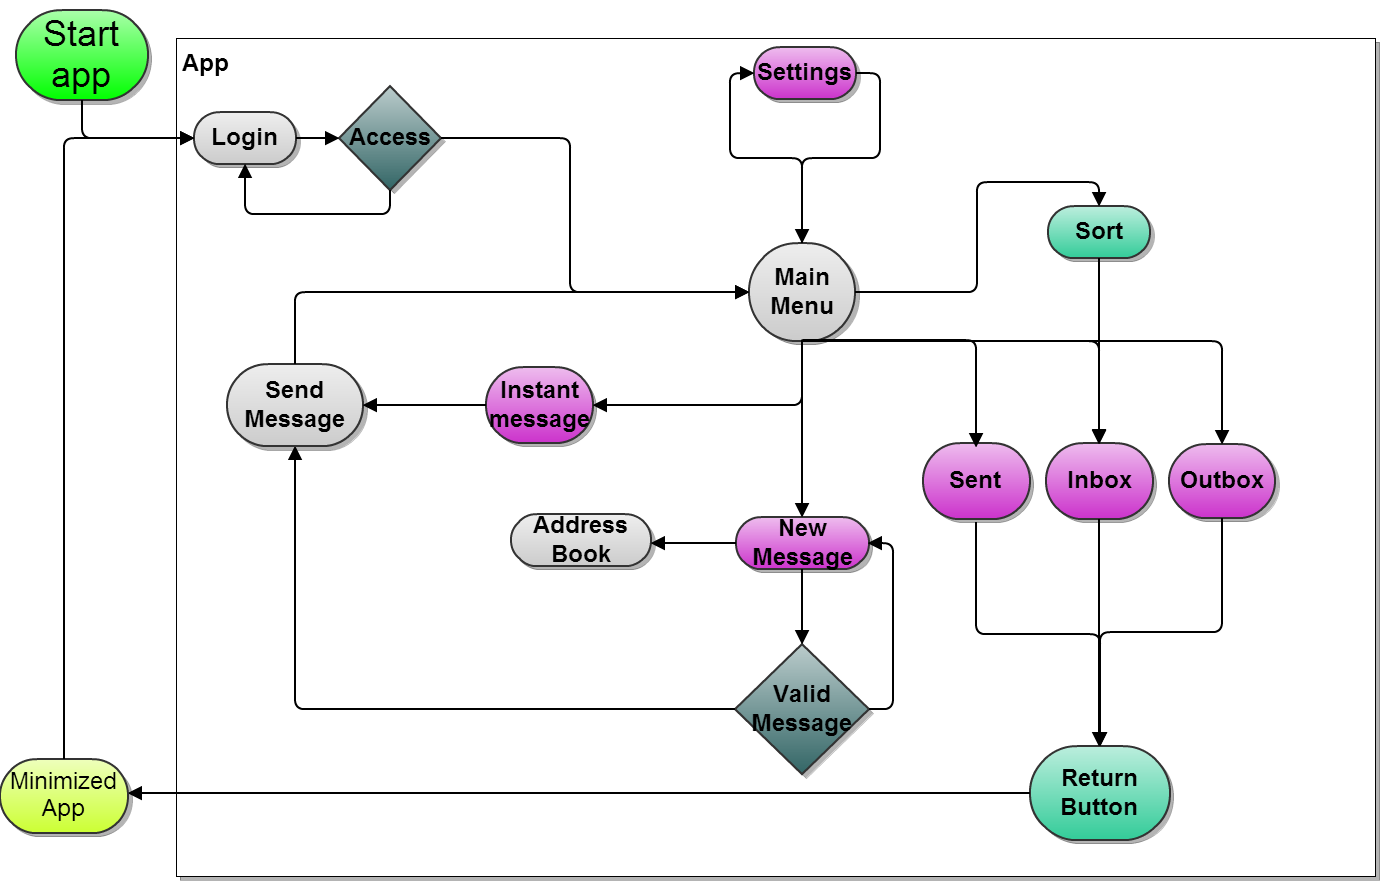
\includegraphics[width=\textwidth]{activities_flowchart3}
	\caption{The activity flow for XOXOmail}
	\label{fig:logicalGUIview}
\end{figure}

Figure \ref{fig:logicalGUIview} at page \pageref{fig:logicalGUIview} shows the flow in our application. The entry point for our application is shown at the upper left corner at "Start app". The first activity you see is the \textsc{Login Activity}. The user is granted access if a correct username and matching password is entered. He is then sent directly to the main menu, where he can choose to either see messages, send a new message or alter settings. Which messages are shown are based on if you choose \highlight{Sent} or \highlight{Inbox}. By pressing \highlight{Sort} he can choose to alter the way the messages are shown. Choosing to send a message can either be done by going into the regular send message view, or the instant message view. Either way, for a message to be sent, it has to be validated. When all fields are valid, the message is sent to the correct recipient. By pressing return button when inside application we are minimizing the application, it will however still be running in the background.

\newpage

\section{Architectural tactics}
	This section will in general be a discussion about and around tactics found in 'Software Architecture in Practice'\cite{bib:archi}. 
	\subsection{Security}
		Tactics for ensuring the security of an application and its data is of often divided into three seperate ways of operating, resisting attacks, detecting attacks and recovering from an attack. 
		In the case of XOXOmail, resisting attacks will be the main focus. As seen in figure~\ref{fig:securityview} on page~\pageref{fig:securityview}, we have opted for a layered security architecture in order to best secure the application data. In terms of what is listed in 'Software Architecture in Practice'\cite[p. 119]{bib:archi}, XOXOmail will in one way or another touch upon all of the six tactics listed. 

\newpage

		\begin{description}
			\item[Authenticate Users] XOXOmail will keep a users credential stored after the first time login. The first time login authentication procedure consists of trying to login to mail gateway.
			\item[Authorize Users] After authenication, a folder is allocated for the user. All data within this folder will be encrypted using a derivative of the users password. 
			\item[Maintain data confidentiality] The local data storage will be secured by encryption, as described in the previous point. Network is encrypted using \gls{ssl}. 
			\item[Maintain Integrity] Data integrity is a concern at three points: when updating of a model, storing data and network communication. Data integrity when updating a model will be assured by encapsulation, network communication will be secured by \gls{ssl} running on top of \gls{tcp}, the message content will in addition be signed using \gls{emims}. For the storing of data the \highlight{PersistenceService} should ensure the data integrity by conforming to the \gls{acid} properties.
			\item[Limit Exposure] The exposure of services within XOXOmail is limited by the authenication of user, since no services are available before the user is successfully authenticated.
			\item[Limit access] Access can be gained to data in two separate ways, and XOXOmail tries to prevent both. In the case of physical access to the device, an authentication process must be completed. Attempting to gain access through network communication will be prevented by a trust manager, only accepting connections to gateways with a known certificate. 
		\end{description}
		
	\subsection{Usability}
		``Usability is concerned with how easy it is for the user to accomplish a desired task and the kind of user support the system provides.''\cite[p. 90]{bib:archi} The paragraph goes on to explain areas of interest like; learnability, efficiency, error prevention, system adaptations and user confidence and satisfaction. Though usability itself has few tactics that can be implemented directly, there are some general stategies as to how a designer can increase each of these areas quantitative value, as seen in table \ref{tab:uidesign} on page \pageref{tab:uidesign}. 
		
		\begin{table}[H]
		\begin{description}
			\item[Consistency of data display] Terminology, abbreviations, formats, colors and so on should be standardized.
			\item[Efficient information assimilation by the user] The format should be familiar to the user. 
			\item[Minimal memory load on the user] Users should not be required to remember information from one screen for use on another screen.
			\item[Compatibility of data display with data entry] The format of displayed information should be linked clearly to the format of the data entry.
			\item[Flexibility for user control of data display] Users should be able to get the information from the display in the form most convenient for the task on which they are working.
		\end{description}
		\caption{Paraphrased table from 'Designing the User Interface'\cite[p. 77]{bib:uidesign}}
		\label{tab:uidesign}
		\end{table}

\newpage

		In most cases making a good user interfaces requires several iterations with designing and testing. Hence a easily modifiable user interface is preferred, this can be achived by separating the user interface from the rest of the application. This separation can be achived by numerous tactics, most known is perhaps the Model-View-Controller pattern. Though not directly applicable to the Android platform, it carries some general principles which can be used in order to achive the general notion of a MVC architecture. 
		
	\subsection{Modifiability}
		Even though modifiability was not one of the choosen quality attributes, it has had a significant impact on the overall architecture and is therefore included here. From 'Software Architecture in Practice'\cite[p. 111]{bib:archi} it is listed three main areas for modifiability tactics, which each has several tactics. The ones used by XOXOmail are listed in table~\ref{tab:modtac} on page~\pageref{tab:modtac}.
		\begin{table}[H]
			\begin{description}
				\item[Localize change] In an attempt to maximize the systems functional cohesion several tactics where utilized. The services in XOXOmail utilizes a tactic known as \textsc{Generalize Module} as it uses dependency injection instead of multiple fairly similar functions. This allows for a more general use of the module by changing the input parameters to it, instead of the module itself. Another tactic used is \textsc{abstract common services}, which can be seen on both the frontend and backend part of the application. Frontend, all activities inherit from a wrapper class which manages the connection to the backendservice. Backend, all services inherit from an abstract service which manages all commonalities between each service. 
				\item[Prevention of ripple effect] The prevention is done by the use of interfaces, supplemented by a factory pattern for easy creating of services. 
				\item[Defer binding time] The concept of configuration files is utilized by XOXOmail when the application is first starting up. The user also has the possibility to change the configuration files through the user interface, and thus making the application fit the users needs. 
			\end{description}
			\caption{Modifiability tactics in use in XOXOmail}
			\label{tab:modtac}
		\end{table}
		
	\subsection{Testability}
		One of the problem with testing when creating an Android application is the Android dependent code and long build-test-cycle time, which in many cases discourages testing. As a biproduct of the tactics mentioned in the previous sections, both these problems were handled. By keeping the modules as close to pure Java as possible it is possible to run tests locally on your computer, without the need of compiling the complete application and deploying it to the phone, which in turn greatly reduces the build-test-cycle time. This was of course made possible through very generalized modules, were most dependency were injected into the module. 
		
\section{Architectural patterns}
	XOXOmail is built up of several architectural pattern working together to create the best possible experience for every stakeholder involved in this project. The most prominent being our own derivation of the Model-View-Controller pattern, where the whole frontend has taken the part of being a view-controller, and the backend service a pure controller. A great amount of modifiability is achived with this pattern, and by using interfaces to describe modules and their respective callbacks. 
	
\section{The sequence of operations}
	The sequence diagrams below show the general sequence of executed methods when the application is running normally. It is however somewhat simplified in order to best convey the general notion of the sequence, this is due to the fact that the implementation uses multiple concurrent threads, and callbacks instead of return values to methods. 
	\subsection{The login sequence}
	The key element in the login sequence is the query to the \highlight{UserManager} object, which allows for offline login to the application. This is however only possible if the user has been logged in on that particular device before. In the case that a user has never logged in before, the gateway server is used to verify the user credentials, they are then stored if they are correct. 
	\begin{figure}[H]
		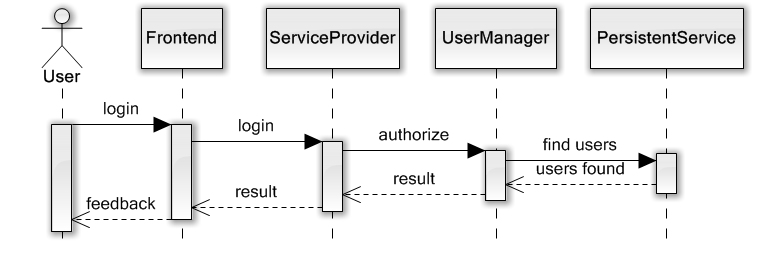
\includegraphics[width=\textwidth]{LoginSequence}
		\caption{The login sequence}
		\label{fig:lifecycle}
	\end{figure}

\newpage
	
\subsection{The send message sequence}
	In this sequence diagram you see the general flow when sending a message. One thing to note is the \highlight{reportMessage}s in the diagram, these are implemented as callback functions in XOXOmail. The reasoning for this is that every time consuming task run in a separate thread, hence a introducing the need for asynchronous callbacks. These callbacks follows the \highlight{Observable pattern}\cite{bib:observer}, which allows for multiple observers. 
	\begin{figure}[H]
		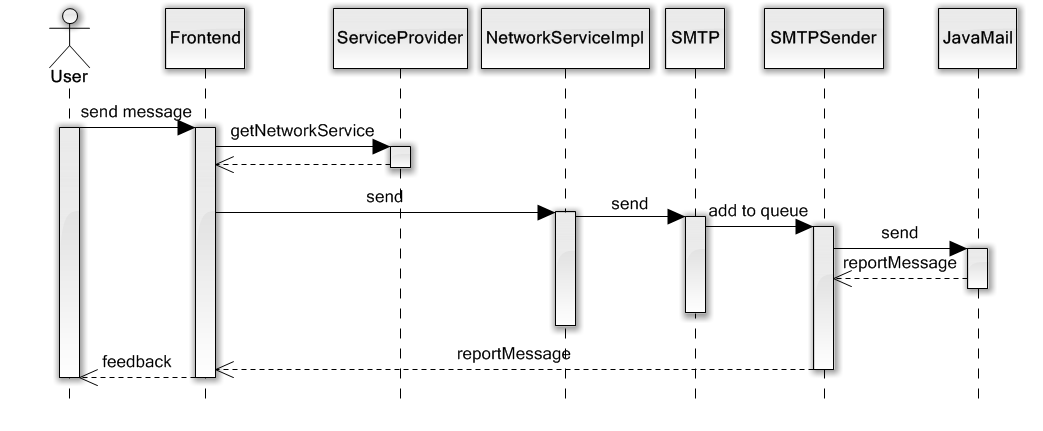
\includegraphics[width=\textwidth]{SendSequence}
		\caption{The send message sequence}
		\label{fig:lifecycle}
	\end{figure}
\subsection{The retrieve message sequence}
	The sequence diagram for retrieving messages show the general setup of the \gls{imapi} strategy. The thing to notice here is the loop structure within the sequence diagram, this is to illustrate the continuality of the idle command issued to the server. 
	\begin{figure}[H]
		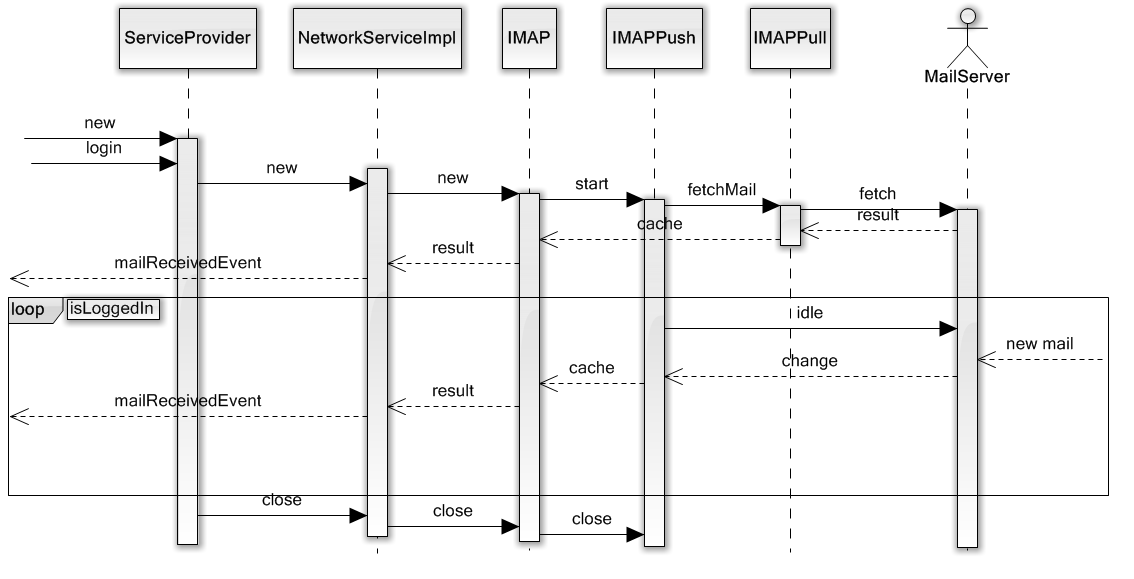
\includegraphics[width=\textwidth]{IMAPPushSequence}
		\caption{The imap push sequence}
		\label{fig:lifecycle}
	\end{figure}
	
